In \autoref{abb:ProdukteDB} werden verwendbare Dienste für die Batch (\enquote{\ac{OLAP}}) Verarbeitung von \ac{AWS}, gemeinsam mit ihren jeweiligen Einsatzgebieten gezeigt. In diesem Abschnitt soll besonders auf die Dienste zur Verarbeitung nach dem Laden der Daten in eine der gezeigten Datenquellen eingegangen werden. Gezeigt werden jedoch auch Dienste für Datenvisualisierung und Machine Learning, da diese komplementär oder mit den prozessierten Daten verwendet werden können. Da die einzelnen Datenquellen jeweils verschiedene Sprachen, bzw. Dialekte von \ac{SQL} verwenden, sind die spezifischen Abfragesprachen mit einem generischen Eintrag in der Grafik abgebildet. Dabei ist es bei \ac{AWS} durchaus üblich, Interoperabilität zu anderen \ac{AWS} Diensten, wie beispielsweise Lambda, in den jeweiligen \ac{SQL} Dialekt einzubauen.

\begin{figure}[H]
\centering
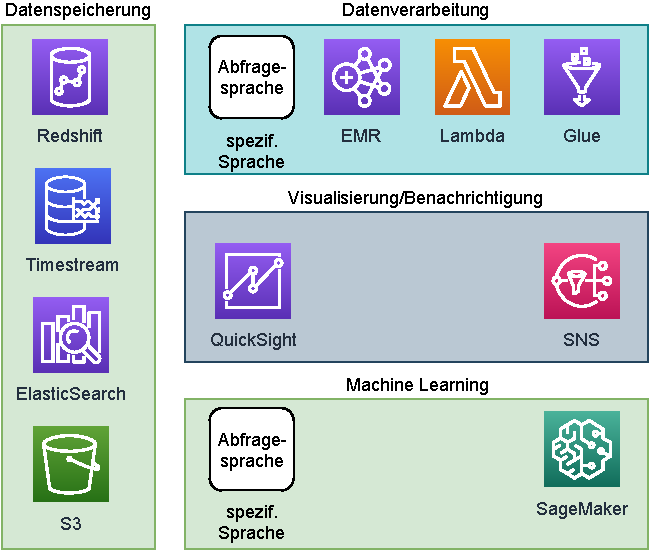
\includegraphics[width=\textwidth]{graphics/Overview-DB.pdf}
\caption{Einsetzbare Produkte im Bereich Datenbankverarbeitung}
\label{abb:ProdukteDB}
\end{figure}


\subsection{Amazon Timestream}






\subsubsection{Produkteinführung}
Timestream ist nach Aussage des Herstellers eine schneller, skalierbare und speziell für Zeitreihendaten entwickelte Datenbank, welche über \ac{AWS} als Dienstleistung bezogen werden kann.\footcite[Vgl. auch im Folgenden][]{AmazonWebServicesInc..o.J.h} Timestream integriert zwei verschiedene Speichertypen, nämlich \ac{RAM}-basierten Speicher, in dem Daten auf welche schnell zugegriffen werden sollen gespeichert werden können und Festplatten-basierten Speicher, welcher für historische Daten dienen soll.
Timestream besetzt zusätzlich einen eigenen \ac{SQL}-Dialekt, welcher um Funktionen zur Analyse von Zeitreihendaten erweitert wurde. Ein Beispiel für den Einsatz des \ac{SQL}-Dialekts zur Kalkulation des 99. Perzentils ist in \autoref{lst:sql-timestream} gezeigt.

\begin{listing}[H]
\inputminted[frame=lines,breaklines=true]{sql}{code/timestream-example.sql}
\caption{Berechnung des 99. Perzentils in Timestream}
\label{lst:sql-timestream}
\end{listing}

\begin{table}[H]
\centering
\begin{tabular}{|l|l|l|l|l|}
\hline
DeviceType & measure\_name & binned\_timestamp & avg & p99 \\ \hline
iotDemo & temperature & 2021-02-26 08:00:00.000000000 & 16.51 & 20.1 \\ \hline
iotDemo & temperature & 2021-02-26 16:00:00.000000000 & 18.23 & 19.2 \\ \hline
iotDemo & temperature & 2021-02-25 18:00:00.000000000 & 18.5 & 19.3 \\ \hline
iotDemo & temperature & 2021-02-25 20:00:00.000000000 & 17.3 & 17.8 \\ \hline
\end{tabular}
\caption{Ausgabe der Datenbank bei Eingabe des oben gezeigten SQL-Statements}
\label{tab:AusgabeSQL}
\end{table}
\subsubsection{Featurevergleich} 
\Todo{Erweitern}
Robustness and fault tolerance
Low latency reads and updates
Scalability
Generalization
Extensibility
Ad hoc queries
Minimal maintenance
Debuggability
vorgestellte Auswertungen 
Reusability of processing logic

\subsubsection{Performancevergleich}
\Todo{Performancegarantien}

\subsubsection{Kostenvergleich}
\begin{listing}[H]
\inputminted[frame=lines,breaklines=true]{sql}{code/timestream-threshold.sql}
\caption{Abfrage für Kostenvergleichs Usecase}
\label{listing:timestream-kostenvergleich}
\end{listing}

Timestream ist momentan noch nicht in Frankfurt verfügbar, weshalb die Kosten in der einzigen europäischen Zone mit verfügbarem Timestream, Irland, als Maßstab verwendet werden. Angenommen wird, dass die Daten eine Stunde im \ac{RAM} vorgehalten werden und danach in die Festplattenspeicherung überführt werden.

%  Angenommen 8.640.000 (8,64 GB)/Monat 0,012GB/h 4,885056
% Abfrage: 25,92 GB

Ausgehend von dem beschriebenen Szenario lässt sich nicht genau errechnen, welche Datenmenge von den Anfragen genau erfasst wird. Dies ist dem Fakt geschuldet, dass Timestream die Daten optimiert abspeichert und nur den tatsächlichen Messwert speichert. Numerische Daten können als 32-bit int, als 64bit BigInt oder als 64bit double gespeichert werden.\footcite[Vgl. auch im Folgenden][]{AmazonWebServicesInc..o.J.r}\nzitat\footcite[Vgl. auch im Folgenden][]{AmazonWebServicesInc..o.J.q} Wenn dazu ein String für die Sensorid im Stile \enquote{Sensor-123} angenommen wird, der 19 bytes zur Darstellung benötigt und der Zeitstempel addiert wird, der 8 bytes benötigt, ergibt sich eine Speicherbelegung von 91 Bytes. Speicherkosten werden aber bei Werten unter einem Kilobyte auf einen Kilobyte hochgerundet, weshalb dies in der Speicherrechnung keine Beachtung findet. Wenn man weitere Optimierungen, die die Abfrageengine macht außer Acht lässt, muss mit 0,78624GB pro abgefragtem Monat gerechnet werden.

\Todo{Lambda Orchestration hinzufügen}
\begin{table}[H]
\centering
\begin{tabular}{|l|l|l|}
\hline
Dimension & Preis(\$)/Einheit & Summe (\$) \\ \hline
Schreibzugriffe & 0,5654/Mio./KB & 4,885056 \\ \hline
\begin{tabular}[c]{@{}l@{}}\ac{RAM} \\ Speicherung\end{tabular} & 0,0407/GB/h & 0,351648 \\ \hline
\begin{tabular}[c]{@{}l@{}}Festplatten\\ Speicherung\end{tabular} & 0,0339/GB/Monat & 0,878688 \\ \hline
Anfragen & \begin{tabular}[c]{@{}l@{}}0,011308/GB \\ abgefragt\end{tabular} & 25,6055095296 \\ \hline
Summe &  & 31,7209015296 \\ \hline
\end{tabular}
\caption{Kostenvergleich AWS~Timestream}
\label{tab:kostenvergleich-AWS~Timestream}
\end{table}

\subsubsection{Gesamtbewertung}
\produktbewertung{Amazon~Timestream}{x,10,7,8,7,5,3,4,2,1,0,x}

\subsection{Amazon Athena}\label{chap:athena}

\subsubsection{Produkteinführung}
Amazon Athena ist nach Aussage des Herstellers ein voll verwalteter Query Dienst, welcher das durchsuchen von großen Datenmengen im \ac{S3} Speicherdienst möglich macht.\footcite[Vgl.][]{Barr.2016} Athena basiert dabei auf dem ursprünglich von Facebook entwickelten Presto, welches mittlerweile Open Source ist. Innerhalb von Athena können Daten verschiedener Formate (\ac{CSV}, Apache Parquet, Apache ORC, \ac{JSON}, ...) mittels \ac{SQL} verarbeitet werden. Zusätzlich ist seit November 2020 mittels der sogenannten \enquote{Federated Queries} auch die Abfrage von anderen Datenquellen wie Apache HBase, Amazon Document DB oder von Datenquellen, die durch eigenentwickelte Verbindungselemente verknüpft werden.\footcite[Vgl.][]{AmazonWebServicesInc..o.J.s} Technisch werden diese Federated Queries via Lambda abgewickelt.



Bei verändernden Datenschemata wird empfohlen, den Dienst \ac{AWS} Glue Crawler komplementär einzusetzen, welcher die Schemata aus \ac{S3} automatisch extrahiert und in Athena hinterlegt. Andernfalls können die Schemata auch manuell hinterlegt werden.

\subsubsection{Featurevergleich} 
\Todo{Erweitern}
Robustness and fault tolerance
Low latency reads and updates
Scalability
Generalization
Extensibility
Ad hoc queries
Minimal maintenance
Debuggability
vorgestellte Auswertungen 
Reusability of processing logic

\subsubsection{Performancevergleich}
\Todo{Performancegarantien}

\subsubsection{Kostenvergleich}
Für die Folgende Kostenbewertung wird angenommen, dass Athena die Daten aus \ac{S3} indiziert, welche im \ac{JSON} Format gespeichert werden. Zu beachten ist, dass effizientere Formate wie CSV, oder sogar Apache Parquet und ORC, welche komprimiert Daten speichern können, verwendet werden  könnten. Verwendung von Parquet oder ORC würde laut \ac{AWS} 30-90\% Kosten sparen.\footcite[Vgl.][]{AmazonWebServicesInc..o.J.t} Gleichzeitig kann aber eine Speicherung im \ac{JSON} Format via \AWSIOT{} Rule erfolgen, ohne dass weitere Verarbeitung notwendig ist.

Athena pricing: AmazonWebServicesInc..o.J.t  rounded up to the nearest megabyte, with a 10MB minimum per query
Glue pricing: AmazonWebServicesInc..o.J.u
Step Functions pricing: AmazonWebServicesInc..o.J.v


\begin{figure}[H]
\centering
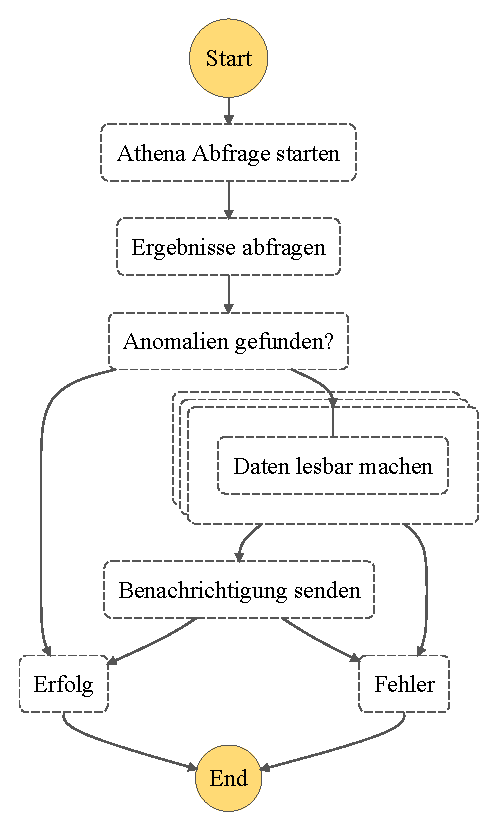
\includegraphics[height=0.45\textheight]{graphics/Step-Function-Athena.pdf}
\caption{Beispiel Step Function State Machine}
\label{abb:StepFunctionExample}
\end{figure}

\begin{table}[H]
\centering
\begin{tabular}{|l|l|l|}
\hline
Dimension & Preis(\$)/Einheit & Summe (\$) \\ \hline
Athena Abfragen & \begin{tabular}[c]{@{}l@{}}0,005/GB \\ abgefragte Daten\end{tabular} &  \\ \hline
\begin{tabular}[c]{@{}l@{}}Glue Data Catalog\\ Speicher\end{tabular} & 1/100.000 Objekte &  \\ \hline
\begin{tabular}[c]{@{}l@{}}Glue Data Catalog\\ Abfragen\end{tabular} & 1/Million Abfragen &  \\ \hline
Step Functions & \begin{tabular}[c]{@{}l@{}}0,025/1000 \\ Zustandsübergänge\end{tabular} &  \\ \hline
\ac{SNS} (Push) & \begin{tabular}[c]{@{}l@{}}0,00002/Nachricht\\ (angenommen 5 Alarme/Gerät/Monat)\end{tabular} & 0,02 \\ \hline
Summe &  &  \\ \hline
\end{tabular}
\caption{Kostenvergleich Amazon~Athena}
\label{tab:kostenvergleich-Amazon~Athena}
\end{table}


\subsubsection{Gesamtbewertung}
\produktbewertung{Amazon~Athena}{x,x,x,x,x,x,x,x,x,x,x,x}


\subsection{Amazon Redshift}

\subsubsection{Produkteinführung}
Amazon Redshift ist der Data Warehouse Dienst von \ac{AWS}, welcher nach Aussage des Herstellers \enquote{enterprise-level} ist und auf ein Datenvolument von Petabytes skalieren kann. \footcite[Vgl.][1]{AmazonWebServicesInc..o.J.g} Redshift ist dabei ein klassisches \ac{OLAP} Produkt, welches für eine Vielzahl verschiedener Daten effizient Auswertungen bereitstellen kann. Redshift basiert auf der bekannten Open Source Datenbank PostgreSQL, weicht jedoch in der Implementierung diverser Kommandos und Features ab, die das Amazon als irrelevant für \ac{OLAP} Anwendungen hält.\footcite[Vgl.][4]{AmazonWebServicesInc..o.J.g}\nzitat\footcite[Vgl.][428\psqq]{AmazonWebServicesInc..o.J.g} Kern von Redshift sind sogenannte Cluster, welche aus einer oder mehrerer Berechnungsknoten (\enquote{compute nodes}) und Anführerknoten(\enquote{leader nodes}) besteht. Applikationen interagieren allein mit den Anführerknoten, die existierenden Berechnungsknoten sind zwar transparent für die Anwendung, werden jedoch von den Anführerknoten mit Ausführungsplänen versorgt, die diese entwickelt um Anfragen effizient zu verarbeiten.\footcite[Vgl.][4]{AmazonWebServicesInc..o.J.g}

Redshift bietet zusätzlich mit Redshift Spectrum einen Dienst an, welcher auf den ersten Blick dem in \autoref{chap:athena} vorgestellten Athena gleicht. Beide rufen via \ac{SQL} Daten von \ac{S3} ab und beide kosten 5\$/TB gescannte Daten.\footcite[Vgl. auch im Folgenden][]{Smallcombe.2020} Wichtige Unterschiede liegen dabei aber in der Art, wie Ressourcen verwaltet und genutzt werden können. Während Redshifft Spectrum nur in Kombination mit einem Redshift Cluster verwendet werden kann, funktioniert Athena ohne Kopplung an verwaltende Ressourcen. Gleichzeitig ist ein stärkerer Einfluss auf die Performance bei Redshift möglich, da man zusätzliche Clusterressourcen einfach provisionieren kann, während Athena vollständig von \ac{AWS} verwaltet wird. Entsprechend erlaubt Redshift Spectrum zwar größeren Einfluss auf die Performance von Datenabfragen, dieser Einfluss muss jedoch in Form von zusätzlich abzurechnenden Clusterressourcen abgerechnet werden, was Redshift für Anwendungsfälle, die keine gesichert gleichbleibende Performance benötigen, unattraktiv macht.


\subsubsection{Featurevergleich} 
\Todo{Erweitern}
Robustness and fault tolerance
Low latency reads and updates
Scalability
Generalization
Extensibility
Ad hoc queries
Minimal maintenance
Debuggability
vorgestellte Auswertungen 
Reusability of processing logic

\subsubsection{Performancevergleich}
\Todo{Performancegarantien}

\subsubsection{Kostenvergleich}
Da Redshift Spectrum durch die zusätzlich zu provisionierenden Clusterresourcen einen Kostennachteil hat, wird von einem Kostenvergleich für Spectrum abgesehen. Stattdessen werden die Kosten für ein Redshift \ac{OLAP} Cluster berrechnet. Dabei ist zu beachten, dass \AWSIOT{} keine direkte Rule bietet, um Daten in Redshift abzulegen. Stattdessen müssen die Daten via Kinesis Data Firehose oder \ac{AWS} Lambda eingefügt werden. Zum Zwecke der Datenübertragung wird in diesem Fall Kinesis Data Firehose kalkuliert. Wie bei Elasticsearch Service gibt es auch bei Redshift verschiedene unterliegende Instanzen zur Auswahl.\footcite[Vgl. auch im Folgenden][]{AmazonWebServicesInc..o.J.z} Im Vergleich werden, den Empfehlungen von \ac{AWS} folgend, eine Instanz der \ac{DC2} Klasse verwendet, welche sich für unkomprimierte Datenmengen kleiner ein TB eignen. Die kleinste verfügbare \ac{DC2} Instanz ist \enquote{dc2.large} mit 2 vCPUs, 15GiB Hauptspeicher und ~160 GB Festplattenspeicher. Redshift muss innerhalb eines \acp{VPC} gestartet werden, um Netzwerkisolation sicherzustellen. Aus diesem Grund muss ein Aufpreis auf Kinesis Data Firehose zu zahlen, welches Datenübertragung in ein \ac{VPC} mit einem Aufschlag berechnet.\footcite[Vgl. auch im Folgenden][]{AmazonWebServicesInc..o.J.y} Kinesis Data Firehose rundet dazu noch Daten zu den nächsten 5 KB auf, was eine effektive Datenmenge von 41,77GB ergibt.

Zusätzlich müssen Lambda Ausführung dazu gerechnet werden, die die Ausführungen der hinterlegten \ac{SQL} Abfragen zur Auswertung ausführen und danach \ac{SNS} benachrichtigen.

\begin{table}[H]
\centering
\begin{tabular}{|l|l|l|}
\hline
Dimension & Preis(\$)/Einheit & Summe (\$) \\ \hline
\begin{tabular}[c]{@{}l@{}}dc2.large Instanz\\ (OnDemand)\end{tabular} & 0,324/h & 233,60 \\ \hline
\begin{tabular}[c]{@{}l@{}}Firehose \\ Dateneingang\end{tabular} & 0,033/GB & 1,38 \\ \hline
\begin{tabular}[c]{@{}l@{}}Firehose\\ \ac{VPC}\end{tabular} & \begin{tabular}[c]{@{}l@{}}0,01/GB\\ 0,012/h\end{tabular} & 8,84 \\ \hline
Lambda Ausführungen & 0,0000002/Ausführung & 0,000192 \\ \hline
Lambda \ac{RAM} & 0,0000000167/GB-Sekunde & 0,08 \\ \hline
\ac{SNS} (Push) & \begin{tabular}[c]{@{}l@{}}0,00002/Nachricht\\ (angenommen 5 Alarme/Gerät/Monat)\end{tabular} & 0,02 \\ \hline
Summe &  & 243,920192 \\ \hline
\end{tabular}
\caption{Kostenvergleich Amazon~Redshift}
\label{tab:kostenvergleich-Amazon~Redshift}
\end{table}



 



\subsubsection{Gesamtbewertung}
\produktbewertung{Amazon~Redshift}{x,x,x,x,x,x,x,x,x,x,x,x}

\subsection{Amazon Elasticsearch}

\subsubsection{Produkteinführung}
Amazon Elasticsearch ist die verwaltetete Variante der ehemals Open-Source Elasticsearch Datenbank, entwickelt von Elastic.\footcite[Vgl.][]{Barr.01.10.2015} Elasticsearch ist dabei nach Aussage des Herstellers eine verteilte, freie und offene Analytics- und Suchplattform für viele verschiedenen Datenformen.\footcite[Vgl.][]{ElasticsearchInc..o.J.} Elasticsearch basiert auf der Open Source Bibliothek Apache Lucene. Elasticsearch geniesst neben der Popularität im Bereich Logverarbeitung und Monitoring auch Beliebtheit als \ac{IIoT} Datenbank.\footcite[Vgl.][]{Mantfeld.2019}\nzitat\footcite[Vgl.][]{Bajer.2017}

\subsubsection{Featurevergleich}
Robustness and fault tolerance
Low latency reads and updates
Scalability
Generalization
Extensibility
Ad hoc queries
Minimal maintenance
Debuggability
vorgestellte Auswertungen 
Reusability of processing logic

\subsubsection{Performancevergleich}
\Todo{Performancegarantien}

\subsubsection{Kostenvergleich}
Der \ac{AWS} Elasticsearch Service wird auf unterliegenden \ac{EC2} Instanzen betrieben und wie diese in gewissen Klassen abgerechnet. Dabei stehen sowohl OnDemand Abrechnugsmodelle wie auch reservierte Kapazität zur Verfügung.\footcite[Vgl. auch im Folgenden][]{AmazonWebServicesInc..o.J.w} Zusätzlicch steht mit \enquote{UltraWarm} eine besondere Instanzklasse zur Verfügung, welche für das Vorhalten großer Datenmengen konzipiert ist. Zusätzlich zu den Instanzen wird noch der verbrauchte \ac{EBS}-Speicherplatz abgerechnet. Dieser Speicherplatz kann in der Standard Klasse oder speziell für hohen Datendurchsatz (provisionierte \ac{IOPS}) gebucht werden. Der Speicherplatz für UltraWarm wird aber nicht via \ac{EBS} abgerechnet, sondern separat. Ebenfalls steht wieder ein \enquote{Free Tier} zur Verfügung, welches aus Vergleichsgründen nicht in die Berechnung einfliessen soll. Aus Vergleichsgründen kommen nur OnDemand abgerechnete Instanzen für den Vergleich in Frage. Für Vergleichszwecke soll eine t3.medium.elasticsearch Instanz geschätzt werden, welche mit 2 vCPUs und 4 GiB \ac{RAM} ausgestattet ist. Der provisionierte \ac{EBS}-Speicherplatz soll bei 10GB liegen.

Benachrichtigungen werden über die native Integration von Kibana und \ac{SNS} abgewickelt, wobei Kibana die Wertüberwachung übernimmt.\footcite[Vgl.][]{AmazonWebServicesInc..o.J.x}

\begin{table}[H]
\centering
\begin{tabular}{|l|l|l|}
\hline
Dimension & Preis(\$)/Einheit & Summe (\$) \\ \hline
\begin{tabular}[c]{@{}l@{}}t3.medium Instanz\\ (OnDemand)\end{tabular} & 0,084/h & 61,32 \\ \hline
\ac{EBS} Speicher & 0,161/GB & 1,61 \\ \hline
\ac{SNS} (Push) & \begin{tabular}[c]{@{}l@{}}0,00002/Nachricht\\ (angenommen 5 Alarme/Gerät/Monat)\end{tabular} & 0,02 \\ \hline
Summe &  & 62,95\\ \hline
\end{tabular}
\caption{Kostenvergleich Amazon~Elasticsearch~Service}
\label{tab:kostenvergleich-Amazon~Elasticsearch~Service}
\end{table}

\subsubsection{Gesamtbewertung}
\produktbewertung{Amazon~Elasticsearch}{x,x,x,x,x,x,x,x,x,x,x,x}

\subsection{Produktauswahl}
\begin{table}[H]
\centering
\begin{tabular}{|l|l|l|}
\hline
Platz & Name & Summe \\ \hline
x & Amazon Timestream & \cellcolor[HTML]{DAE8FC}x \\ \hline
x & Amazon Redshift & \cellcolor[HTML]{DAE8FC}x \\ \hline
% x & Amazon S3 & \cellcolor[HTML]{DAE8FC}x \\ \hline
x & Amazon Athena & \cellcolor[HTML]{DAE8FC}x \\ \hline
x & Amazon Elasticsearch & \cellcolor[HTML]{DAE8FC}x \\ \hline
\end{tabular}
\caption{Produktreihenfolge Batch}
\label{tab:Reihenfolge-Batch}
\end{table}





